\subsection{Predicting vehicle state: the transition function}
\label{sec:vehicle_model_trans}

The goal of the prediction step is to obtain a \emph{prior distribution} of the vehicle's state at time $\Vtime_k$ based on its previous state at time $\Vtime_{k-1}$. That is, we wish to estimate $p(\Vstate_k | \Vstate_{k-1})$. Using the model definition in \cref{eq:vehicle_model} along with the particle filter approximation of state in \cref{eq:vehicle_state_dirac}, we can write the prior prediction of the vehicle's state as
\begin{equation}
\label{eq:vehicle_pf_predict}
p(\Vstate_k | \Vstate_{k-1}) \approx
\sum_{i=1}^\Np
    \Pwt_{k-1}
    \DiracMeasure{\Vstate_k\vi}{\Vstate_k},
\end{equation}
where $\Vstate_k\vi = f(\Vstate\vi_{k-1}, \Vtdiff_k, \Vnoise_k)$ and $\Vtdiff_k = \Vtime_k - \Vtime_{k-1}$.

The transition function $\Vtrans$ is where we define the vehicle behaviours mentioned earlier (and others). In Kalman filter applications, one is limited to linear transformations of the state which can be expressed in a \emph{transition matrix}. However, we see in \cref{eq:vehicle_pf_predict} that, in the particle filter implementation, the transition function is applied to each particle independently, allowing for a lot more flexibility in $\Vtrans$. We now describe the various model components of $\Vtrans$, which we implemented as an algorithm in the \verb+transitr+ package (see \cref{sec:particle-filter} for details). The core components are vehicle motion (speed and acceleration along a known path), stopping behaviour at known locations (bus stops and intersections), and a suite of other scenarios we may need to include to avoid degeneration.


\subsubsection{Component A: vehicle motion}
\label{sec:vehicle_model_behaviour}

The first behaviour to consider is that of any vehicle travelling along a known path: the \emph{speed} at which a vehicle is travelling will affect where it ends up. Since speed, $\Vspeed$, is the derivative of distance travelled over time, that is if $x = d(t)$, then $\Vspeed = d'(t)$, which was shown visually in \cref{fig:vehicle_state}. It follows that we can predict a vehicle's future state, given its current state (distance travelled and speed) and system noise,
\begin{equation}
\label{eq:vehicle_model_newton}
\Vstate_{k|k-1} = f_{A1}\left(\Vstate_{k-1|k-1}\right) =
\begin{bmatrix}
\Vdist_k \\ \Vspeed_k
\end{bmatrix} =
\begin{bmatrix}
\Vdist_{k-1} + \Vtdiff_k\Vspeed_k \\
\Vspeed_{k-1} + v_k
\end{bmatrix},\quad
v_k \sim \TNormal{0}{\Vnoise}{-\Vspeed_{k-1}}{30 - \Vspeed_{k-1}}.
\end{equation}
In this case, the noise term is truncated to ensure the new speed is both positive and under 30~m/s, which is 108~km/h (the maximum road speed in Auckland is 100~km/h)
The resulting transition function, $\Vtrans_{A1}$, can quite simply be implemented by simulating, for each particle, a new speed before calculating the final state using \cref{eq:vehicle_model_newton}. A similar model was used by \citet{Cathey_2003,Dailey_2001}.

% The variance of predicted distance travelled is
% \begin{equation}
% \label{eq:model_a1_var}
% \begin{split}
% \Var{\Vdist_k}
% &= \Var{\Vdist_{k-1} + \Vtdiff_k (\Vspeed_{k-1} + v_k)} \\
% &= \Var{\Vdist_{k-1}} + \Vtdiff_k^2\Var{\Vspeed_{k-1}} +
%     \Vtdiff_k^2\Vnoise
% \end{split}
% \end{equation}

\Cref{fig:transition_a1_demo} demonstrates transition model $\Vtrans_{A1}$ using a sample of $N=10$~particles which, at time $t_{k-1}$, take one of three unique states (due to resampling in the previous iteration). The points have been coloured by this initial state to demonstrate the effect of adding noise \emph{before} transitioning, and how the system noise controls how the state spreads. The interpretation of the noise parameter is \emph{the average change in speed, per second, between vehicle observations}. \textcolor{blue}{[[re-write para]]}

\begin{knitrout}\small
\definecolor{shadecolor}{rgb}{0.969, 0.969, 0.969}\color{fgcolor}\begin{figure}

{\centering 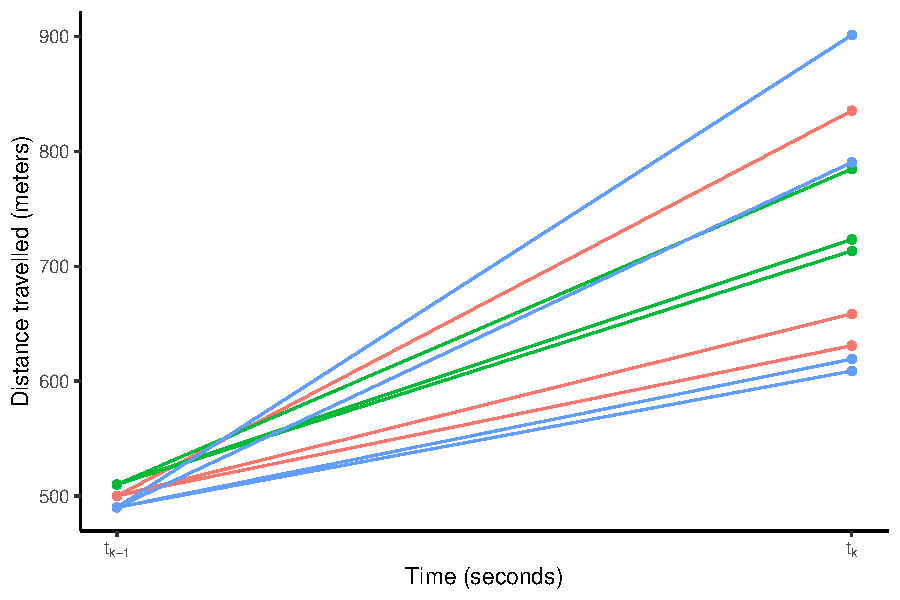
\includegraphics[width=.8\textwidth]{figure/transition_a1_demo-1} 

}

\caption[Simulated particle trajectories using transition model A1]{Simulated particle trajectories using transition model A1. Points have been coloured by their parent (after resampling) to demonstrate the affect of system noise.}\label{fig:transition_a1_demo}
\end{figure}


\end{knitrout}

The main issue with this model is that it assumes constant speed between observations, which---given Auckland traffic---is unlikely to be the case. In \cref{fig:vehicle_state}, we showed speed varying over time, even between observations. To model this, we \emph{iteratively} update the vehicle's state\footnote{This is one advantage of the particle filter---we can easily perform iterative updates!} by reusing \cref{eq:vehicle_model_newton} $\Vtdiff_k$ times, setting $\Vtdiff_k=1$ in each iteration. \Cref{fig:transition_a2_demo} shows the effect this has on the particle's trajectories. Note, however, that in this model the system noise parameter is not the same, and has a slightly different interpretation: it is now \emph{the average change in speed per second} (no longer between observations).

% Under normal circumstances (and without the truncation) the variance of the predicted state is, for $z_m\sim\Normal{0}{\Vnoise}$,
% \begin{equation}
% \label{eq:model_a2_var}
% \begin{split}
% \Var{\Vdist_k}
% &= \Var{\Vdist_{k-1} + \sum_{n=0}^{\Vtdiff_k-1}(\Vspeed_{k-1} +
%     \textstyle\sum_{m=n}^{\Vtdiff_k} z_n)} \\
% &= \Var{\Vdist_{k-1} + \Vtdiff_k \Vspeed_{k-1} +
%     \textstyle\sum_{n=0}^{\Vtdiff_k-1} (\Vtdiff_k - n) z_n} \\
% &= \Var{\Vdist_{k-1}} + \Vtdiff_k^2\Var{\Vspeed_{k-1}} +
%     \Var{\textstyle\sum_{n=0}^{\Vtdiff_k-1} (\Vtdiff_k - n) z_n} \\
% &= \Var{\Vdist_{k-1}} + \Vtdiff_k^2\Var{\Vspeed_{k-1}} +
%     \textstyle\sum_{n=0}^{\Vtdiff_k-1} \Var{(\Vtdiff_k - n) z_n} \\
% &= \Var{\Vdist_{k-1}} + \Vtdiff_k^2\Var{\Vspeed_{k-1}} +
%     \textstyle\sum_{n=0}^{\Vtdiff_k-1} (\Vtdiff_k - n)^2\Vnoise  \\
% &= \Var{\Vdist_{k-1}} + \Vtdiff_k^2\Var{\Vspeed_{k-1}} +
%     \Vnoise \textstyle\sum_{n=1}^{\Vtdiff_k} n^2 \\
% &= \Var{\Vdist_{k-1}} + \Vtdiff_k^2\Var{\Vspeed_{k-1}} +
%     \Vnoise \frac{\Vtdiff_k(\Vtdiff_k+1)(2\Vtdiff_k+1)}{6}
% \end{split}
% \end{equation}
% which grows at a cubic rate, compared to the quadratic rate of $A1$. We must therefore take care when choosing the system noise when $\Vtdiff_k$ is large. To control the variance so it grows more linearly with $\Vtdiff_k$, we can multiply the system noise by $\frac{6\Vtdiff_k^2}{\Vtdiff_k(\Vtdiff_k+1)(2\Vtdiff_k+1)}}$, so now $A1$ and $A2$ have the same variance; however, we will use a larger value of $\Vnoise$ for $A2$ to allow for greater variance of trajectories.

\begin{knitrout}\small
\definecolor{shadecolor}{rgb}{0.969, 0.969, 0.969}\color{fgcolor}\begin{figure}

{\centering 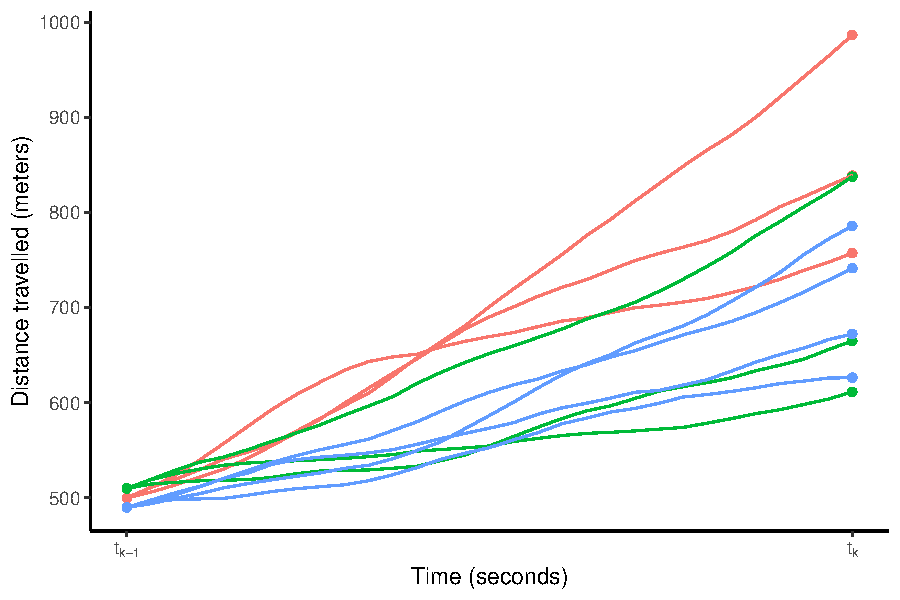
\includegraphics[width=.8\textwidth]{figure/transition_a2_demo-1} 

}

\caption[Simulated particle trajectories using transition model A2]{Simulated particle trajectories using transition model A2. Points have been coloured by their parent (after resampling) to demonstrate the affect of system noise.}\label{fig:transition_a2_demo}
\end{figure}


\end{knitrout}


Of course, if speed is the first derivative of the vehicle's trajectory function, then \emph{accerlation} is the second, $\Vaccel = d''(t)$. In this case, we add a third component to the vehicle's state, and consider speed similarly to distance; the transition function becomes
\begin{equation}
\label{eq:vehicle_model_newton_accel}
\Vstate_{k|k-1} = \Vtrans_{A3}\left(\Vstate_{k-1|k-1}\right) =
\begin{bmatrix}
\Vdist_k \\ \Vspeed_k \\ \Vaccel_k
\end{bmatrix} =
\begin{bmatrix}
\Vdist_{k-1} + \Vtdiff_k\Vspeed_k \\
\Vspeed_{k-1} + \Vaccel_k \\
\Vaccel_{k-1} + v_k
\end{bmatrix}
\end{equation}
with the system noise now applied to the acceleration term and truncated to ensure the speed remains positive and less than 30~m/s,
\begin{equation}
\label{eq:vehicle_model_accel_dist}
v_k \sim \TNormal{0}{\Vnoise}{-\Vspeed_{k-1} - \Vaccel_{k-1}}{30 - \Vspeed_{k-1} - \Vaccel_{k-1}}
\end{equation}
Again, we have displayed the resulting trajectories in \cref{fig:transition_a3_demo}. The main issue is that it is difficult to parameterize and constrain the acceleration to ensure speed remains in the desired region, \emph{and} that the function can still generate plausible trajectories.


\begin{knitrout}\small
\definecolor{shadecolor}{rgb}{0.969, 0.969, 0.969}\color{fgcolor}\begin{figure}

{\centering 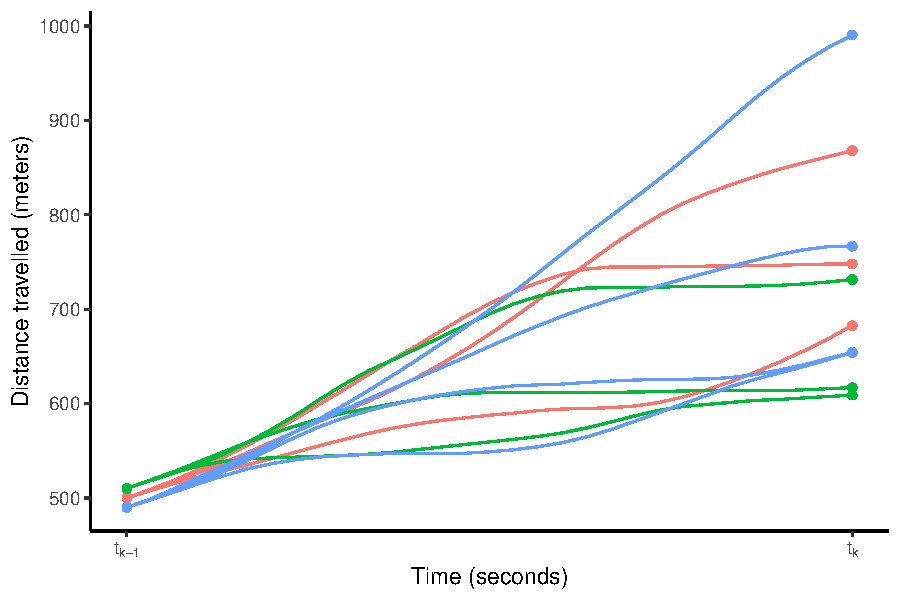
\includegraphics[width=.8\textwidth]{figure/transition_a3_demo-1} 

}

\caption[Simulated particle trajectories using transition model A3]{Simulated particle trajectories using transition model A3. Points have been coloured by their parent (after resampling) to demonstrate the affect of system noise.}\label{fig:transition_a3_demo}
\end{figure}


\end{knitrout}


\subsubsection{Component B: stopping at nodes}
\label{sec:vehicle_model_nodes}

In \cref{sec:route-segments}, we created a road network consisting of nodes---either bus stops or intersections---and the roads connecting them. As a result of this \emph{segementisation}, each route can be expressed as a \emph{sequence of nodes} and connecting \emph{road segments}, as demonstrated in \cref{fig:route-nodes}. Component A of the transition model dealt with vehicle behaviour along the road segments; we now handle the behaviour at these node points.

\begin{knitrout}\small
\definecolor{shadecolor}{rgb}{0.969, 0.969, 0.969}\color{fgcolor}\begin{figure}

{\centering 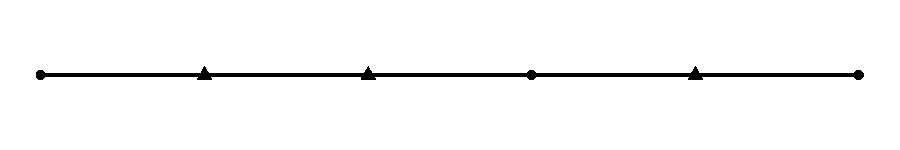
\includegraphics[width=.8\textwidth]{figure/route-nodes-1} 

}

\caption[A simplified route network, showing stops (circles) and intersections (triangles)]{A simplified route network, showing stops (circles) and intersections (triangles).}\label{fig:route-nodes}
\end{figure}


\end{knitrout}

There are two types of nodes in our framework: \emph{bus stops} where passengers can board and disembark, and \emph{intersections} where buses (and other road users) wait depending on congestion levels and traffic lights (we do not distinguish between these currently). In each case, the bus' behaviour is
\begin{enumerate}
\item if the bus stops:
    \begin{enumerate}
    \item deceleration to zero,
    \item wait,
    \item acceleration to traffic speed;
    \end{enumerate}
\item otherwise, continue as though there is no node.
\end{enumerate}
Only step 1b depends on the type of node.



\paragraph{Bus stops}

A bus' wait time at a bus stop is referred to as \emph{dwell time} and consists of three phases (as described by \citet{Hans_2015}):
\begin{enumerate}[i.]
\item doors open
\item passengers board and alight
\item doors close, and vehicle waits for a gap in the traffic\footnote{In New Zealand, buses do not get right-of-way, so it is common for them to be stuck for a while in a bus bay}.
\end{enumerate}
Phases i and ii are combined with 1a and 1c from above (deceleration and acceleration, respectively) into a single parameter, $\mindwell$, which is assumed constant across all buses, stops, and routes.


The service (phase ii) is the time taken for passengers to get on and off the bus, which varies significantly between stop, route, and time of day. There are many ways to model service time, from a simple exponential \citep{Hans_2015} to more complex regression models incorporating real-time passenger demand \citep{Shen_2013} or a real-time Kalman filter \citep{Shalaby_2004}. Here, we present using a truncated normal distribution using the mean and variance of dwell times, truncated at zero. The service time at stop $m$ stop along a route ($m=1,...,M-1$, as dwell time doesn't apply for the last stop) is denoted $\pdwell_m$, which we model by its mean and variance, $\dwell_m$ and $\dwellvar_m$, respectively, estimated from historical data:
\begin{equation}
\label{eq:stop_dwell_time}
\pserve_m \sim \TNormal{\dwell_m}{\dwellvar_m}{0}{\infty}
\end{equation}

For each bus stop, we also have a \emph{stopping probability} $\Prstop_m\in(0,1)$. For the first and last stops, $m\in\{1,M\}$, the is unity; for the remainder, we have no data with which we can reliably estimate $\Prstop_m$, so, for now, we assume all stops have the same values specified by a global $\Prstop$ parameter (see \cref{sec:pf_params} for details on this). The outcome of whether or not a bus stops at a bus stop, $p_m$, is thus a Bernoulli trial,
\begin{equation}
\label{eq:stop_pstop}
\Istop_m \sim \Bern{\Prstop_m}
\end{equation}
The total dwell time of a bus at stop $m$ can be expressed as
\begin{equation}
\label{eq:stop_total_dwell_time}
\pdwell_m = \Istop_m (\mindwell + \pserve_m)
\end{equation}
which, under the particle filtering framework, is straightforward to implement. \Cref{fig:eta_dwell_times} demonstrates the dwell time distribution at a stop.

One other scenario for bus stops is a \emph{layover}, which is when a bus arrives early at a major stop\footnote{This is more common on longer routes in an attempt to keep them to schedule} and waits until the scheduled departure time. In the GTFS stop times table, layovers are denoted by an arrival time early\footnote{This is usually a one-second difference} than the corresponding departure time, as shown in \cref{tab:layover_times}. Again, under the particle filtering framework, this is simple enough to implement: if the particle arrives early, wait until the scheduled departure time before leaving (i.e., adjusting the dwell time). However, it is not always the case that buses will wait for the layover, so we add a probability of adherence, similar to the stopping probability in \cref{eq:stop_pstop}.

\begin{knitrout}\small
\definecolor{shadecolor}{rgb}{0.969, 0.969, 0.969}\color{fgcolor}\begin{table}

\caption{\label{tab:layover_times}Arrival times for a trip with layover stops marked with an asterix ($\star$).}
\centering
\fontsize{8}{10}\selectfont
\begin{tabular}[t]{rll}
\toprule
Stop & Arrives & Departs\\
\midrule
1 & 19:30:00 & 19:30:00\\
2 & 19:30:36 & 19:30:36\\
3 & 19:31:33 & 19:31:33\\
4 & 19:32:04 & 19:32:04\\
5 & 19:32:59 & 19:33:00 *\\
6 & 19:33:42 & 19:33:42\\
7 & 19:34:14 & 19:34:14\\
\bottomrule
\end{tabular}
\end{table}


\end{knitrout}


\begin{knitrout}\small
\definecolor{shadecolor}{rgb}{0.969, 0.969, 0.969}\color{fgcolor}\begin{figure}

{\centering 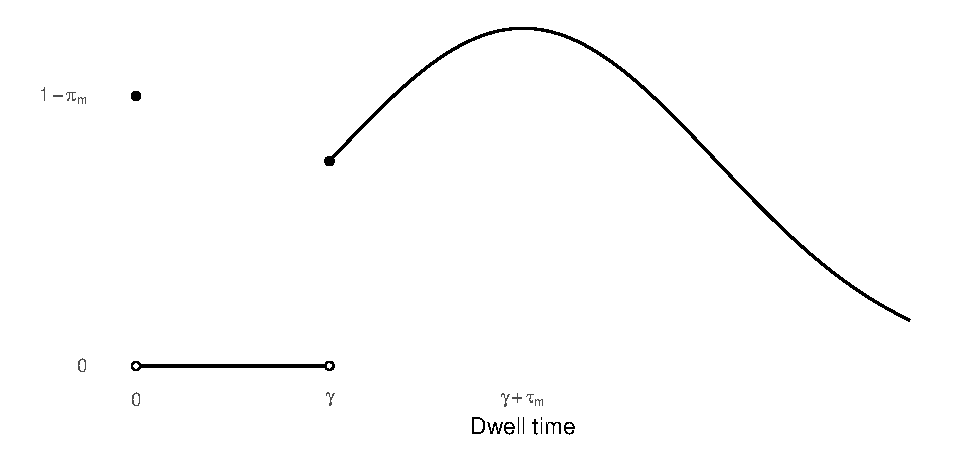
\includegraphics[width=.8\textwidth]{figure/eta_dwell_times-1} 

}

\caption[The \gls{pdf} of dwell time at a stop]{The \gls{pdf} of dwell time at bus stop $m$.}\label{fig:eta_dwell_times}
\end{figure}


\end{knitrout}



\paragraph{Intersections}

Modelling intersections is much the same as bus stops, with a few differences:
\begin{enumerate}[i.]
\item the bus doors do not open, passengers do not get on or off, so there's no longer any $\gamma$ parameter;
\item the bus does not necessarily stop at the node location, since there may be a queue;
\item depending on the length of the queue and the type of intersection, the bus may require more than one "phase" to pass through the intersection (for traffic lights), OR the bus may creep forward slowly (at uncontrolled, give-way intersection or roundabouts).
\end{enumerate}

However, we did not have any reliable intersection location information available, so were unable to explore this component of the model fully. Instead, we describe here a single behaviour but note that it could easily be modified in future.

We model the wait time $w$ at intersection $\ell$ with an exponential distribution with rate $\intwait_\ell^{-1}$:
\begin{equation}
\label{eq:int_wait}
\pcwait_\ell \sim \Exp{\intwait_\ell^{-1}}
\end{equation}
As with bus stops, the stopping outcome $\Iint_\ell$ is a Bernoulli trial with probability $\rho_\ell$,
\begin{equation}
\label{eq:int_stop_bern}
\Iint_\ell \sim \Bern{\rho_\ell}
\end{equation}
which leads to an overall wait time of
\begin{equation}
\label{eq:int_total_wait}
\pwait_\ell = \Iint_\ell \pcwait_\ell
\end{equation}
However, from point iii above, once the wait time is over, we conditionally allow the bus to move forward with the possibility of stopping again. In practice, this would be proportional to the distance of the vehicle from the intersection and other factors. As mentioned in \cref{sec:vp_data}, this is not as easy as it seems since observations may be linked to a waypoint at the intersection\footnote{Actually, in the middle of it} instead of where the bus is, so we cannot determine the bus' distance from the intersection reliably.
